\documentclass{article}
\usepackage{graphicx}
\usepackage{amsmath}
\usepackage{geometry}
\geometry{letterpaper, margin=1in}

\title{EMCH 371 – Fall 2024\\ Homework for Chapter 2}
\date{Due by Tuesday 9/17. Total: 50 Points}
\author{J. Vaught}

\begin{document}
\maketitle

\section*{Problem 1 (Total: 10 Points)}
Schematically plot the net bonding force and bonding energy curves versus interionic separation distance for two isolated ions (e.g., Na\textsuperscript{+} and Cl\textsuperscript{-}).

Please label the equilibrium ion separation distance (i.e., the equilibrium bond length $a_0$), the equilibrium bonding force, as well as the bonding energy at the equilibrium bond length on the plots.
\begin{figure}[h]
	\centering
	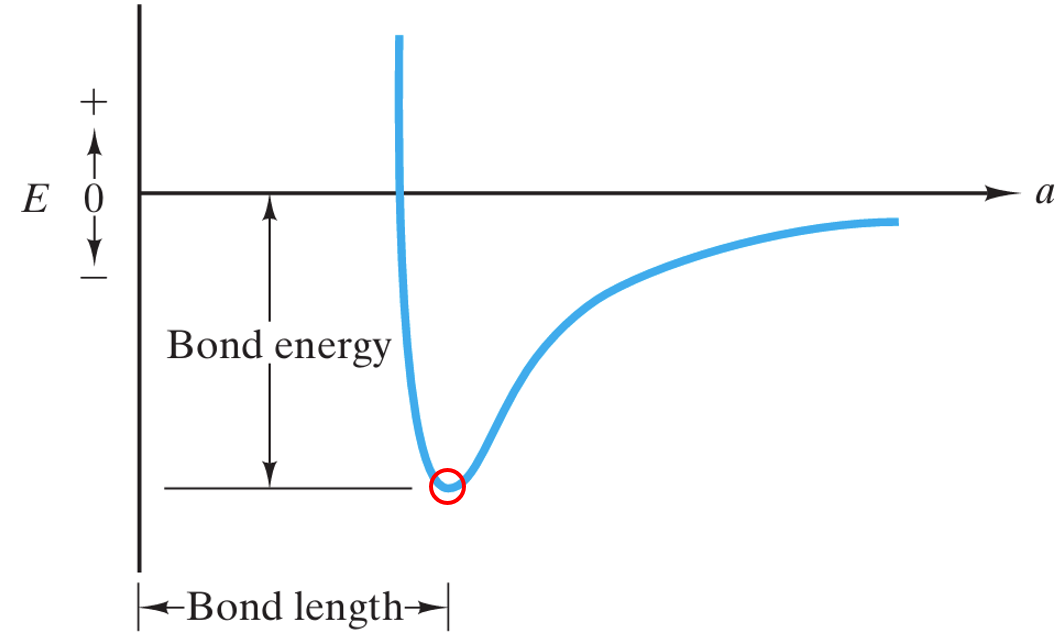
\includegraphics[width=0.7\textwidth]{image1.png} % Replace with the path to your Bonding Energy Curve image
	\caption{Bonding Energy Curve}
\end{figure}

\begin{figure}[h!]
	\centering
	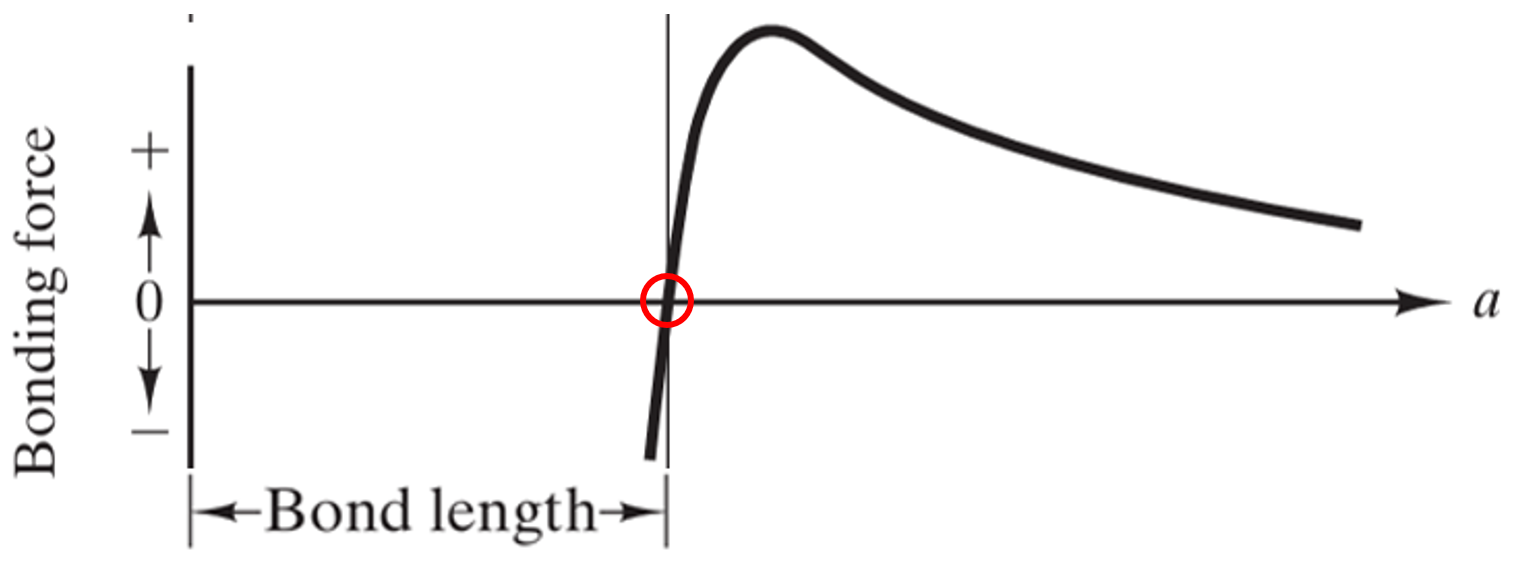
\includegraphics[width=0.6\textwidth]{image2.png} % Replace with the path to your Bonding Force image
	\caption{Bonding Force Curve}
\end{figure}

\newpage
\section*{Problem 2 (Total: 20 Points, 2 Points Each)}
\begin{enumerate}
	\item[(a)] What are the primary bonding types?
	      \begin{itemize}
	      	\item The primary bonding types are ionic, covalent, and metallic bonds. This is discussed in \textbf{Chapter 2, Section 2.1 (Page 23)}.
	      \end{itemize}
	      
	\item[(b)] Which bonding types involve electron transfer?
	      \begin{itemize}
	      	\item Ionic bonds involve electron transfer, where electrons are transferred from one atom to another, creating ions. This is explained in \textbf{Section 2.2 (Page 29)}.
	      \end{itemize}
	      
	\item[(c)] Which bonding types involve electron sharing?
	      \begin{itemize}
	      	\item Covalent and metallic bonds involve electron sharing:
	      	      \begin{itemize}
	      	      	\item Covalent bonds involve the direct sharing of valence electrons between atoms and are highly directional. This is detailed in \textbf{Section 2.3 (Page 41)}.
	      	      	\item Metallic bonds involve electron sharing in the form of delocalized electrons, which allows them to move freely throughout the metal lattice, creating a non-directional bond. This is discussed in \textbf{Section 2.4 (Page 47)}.
	      	      \end{itemize}
	      \end{itemize}
	      
	\item[(d)] Which bonding types involve cooperative sharing of valence electrons?
	      \begin{itemize}
	      	\item Covalent bonds involve cooperative sharing of valence electrons, as described in \textbf{Section 2.3 (Page 41)}.
	      \end{itemize}
	      
	\item[(e)] Which bonding types involve sharing of delocalized valence electrons?
	      \begin{itemize}
	      	\item Metallic bonds involve the sharing of delocalized electrons among a lattice of metal atoms, explained in \textbf{Section 2.4 (Page 47)}.
	      \end{itemize}
	      
	\item[(f)] Which bonding types involve directionally sharing of valence electrons?
	      \begin{itemize}
	      	\item Covalent bonds are directional because they involve specific orbital overlap between atoms, as explained in \textbf{Section 2.3 (Page 41)}.
	      \end{itemize}
	      
	\item[(g)] Which bonding types are directional?
	      \begin{itemize}
	      	\item Covalent bonds are directional, as covered in \textbf{Section 2.3 (Page 41)}.
	      \end{itemize}
	      
	\item[(h)] Which bonding types are non-directional?
	      \begin{itemize}
	      	\item Ionic and metallic bonds are non-directional. Ionic bonds' non-directionality is covered in \textbf{Section 2.2 (Page 30)}, and metallic bonds in \textbf{Section 2.4 (Page 47)}.
	      \end{itemize}
	      
	\item[(i)] Which bonding types have neither electron transfer nor electron sharing?
	      \begin{itemize}
	      	\item Van der Waals (secondary) bonds involve neither electron transfer nor sharing, discussed in \textbf{Section 2.5 (Page 50)}.
	      \end{itemize}
	      
	\item[(j)] Which bonding types tend to have high coordination numbers?
	      \begin{itemize}
	      	\item Ionic and metallic bonds tend to have high coordination numbers due to their non-directional nature, covered in \textbf{Section 2.2 (Page 30)} and \textbf{Section 2.4 (Page 47)}.
	      \end{itemize}
	      
\end{enumerate}

\newpage
\section*{Problem 3 (Total: 10 Points)}
\begin{enumerate}
	\item[(a)] Ions in solids with ionic bonding tend to have the greatest coordination number as geometrically allowable. Why? (3 Points)
	      \begin{itemize}
	      	\item In ionic bonding, the coordination number is determined by the radius ratio of the cation to the anion, which dictates how closely packed the ions can be without repulsive overlap. The ions arrange themselves to maximize electrostatic attraction while minimizing repulsion. Because ionic bonds are nondirectional, ions can surround each other as fully as the geometry allows, leading to high coordination numbers, such as 6 in NaCl and up to 12 in idealized structures. This is covered in \textbf{Section 2.2 (Page 35)}.
	      \end{itemize}
	      
	\item[(b)] Metals tend to have a high coordination number. Why? (3 Points)
	      \begin{itemize}
	      	\item Metals have high coordination numbers because metallic bonds are nondirectional, allowing atoms to pack closely together. The delocalized "sea" of electrons provides cohesive energy uniformly around each atom, which supports high coordination structures like body-centered cubic (coordination number 8) and face-centered cubic (coordination number 12). Efficient packing maximizes the number of neighboring atoms. This is explained in \textbf{Section 2.4 (Page 47)}.
	      \end{itemize}
	      
	\item[(c)] Atoms in solids with covalent bonding tend to have relatively low coordination numbers. Why? (4 Points)
	      \begin{itemize}
	      	\item Covalent bonds are highly directional, as they result from specific orbital overlaps, such as sp³ hybridization in carbon atoms, leading to tetrahedral structures with a coordination number of 4. The directionality limits the number of atoms that can surround a central atom without distorting the bond angles. For example, in diamond, each carbon atom bonds to only four others despite having a radius ratio that could allow more in an ionic setting. This is discussed in \textbf{Section 2.3 (Page 41-43)}.
	      \end{itemize}
	      
\end{enumerate}

\section*{Problem 4 (Total: 10 Points)}
\begin{enumerate}
	\item[(a)] Ceramics and glasses tend to have which types of bonding? (3 Points)
	      \begin{itemize}
	      	\item Ceramics and glasses primarily involve \textbf{ionic bonding} but usually have a significant \textbf{covalent character} as well. Ionic bonds occur due to electron transfer between metal and nonmetal atoms, leading to a strong, non-directional bonding structure. The covalent character comes from the sharing of electrons in specific directions, contributing to the material's rigidity and brittleness. This bonding combination gives ceramics their high melting points, hardness, and electrical insulating properties. This is discussed in \textbf{Section 2.6 (Page 54)}.
	      \end{itemize}
	      
	\item[(b)] Polymers (plastics) tend to have which types of bonding? (4 Points)
	      \begin{itemize}
	      	\item Polymers involve \textbf{strong covalent bonds} along their polymeric chains, which provide strength and structural integrity. However, polymers also exhibit \textbf{weaker secondary bonding} (van der Waals forces) between adjacent chains, which serve as weak links, contributing to lower melting points and mechanical strengths. This combination of bonding types allows polymers to be lightweight, flexible, and easily moldable. This information is covered in \textbf{Section 2.6 (Page 54)}.
	      \end{itemize}
	      
	\item[(c)] Metals tend to have which type of bonding? (3 Points)
	      \begin{itemize}
	      	\item Metals are characterized by \textbf{metallic bonding}, which involves the sharing of delocalized valence electrons among a lattice of metal atoms. These electrons form a "sea" that moves freely, allowing metals to conduct electricity and heat effectively. The nondirectional nature of metallic bonding enables high coordination numbers and closely packed structures, resulting in malleability and ductility. This is explained in \textbf{Section 2.4 (Page 47)}.
	      \end{itemize}
	      
\end{enumerate}

\end{document}